\documentclass[12pt]{article}
\usepackage[portuguese, brazilian, english]{babel}
\usepackage[utf8]{inputenc}
\usepackage[usenames,dvipsnames]{color}
\usepackage{setspace}
\usepackage{amsmath}
\usepackage{amsfonts}
\usepackage{amssymb}
\usepackage{mathtools}
\usepackage[top=3cm, bottom=2cm, left=3cm, right=2cm]{geometry}
\usepackage{tikz}
\usepackage{textcomp}
\usepackage{lscape}    % for landscape pages
\usepackage{hyperref}  % to allow hyperlinks
\usepackage{booktabs}  % nicer table borders
\usepackage{graphicx, subfigure} % add subfigures
\usepackage{rotating}  % sideways figure
\usepackage[verbose]{placeins} % avoids placing figures on last page

    

\title{Projeto MSc}

% Figures directory
\graphicspath{{./figures/}} 

\definecolor{myblue}{RGB}{80,80,160}
\definecolor{mygreen}{RGB}{80,160,80}
\setstretch{1.5}

\begin{document}

% FAPESP demands the usage of double spacing
%
\doublespacing

\selectlanguage{brazilian}
\thispagestyle{empty} 
\begin{flushright}
    {\LARGE Identificação de vias de sinalização celular baseada em repositórios de cinética de reações bioquímicas}

  \bigskip
  \bigskip
        
  {\large {\bf Bolsista:} \href{mailto:gustavo.estrela.matos@usp.br}{Gustavo Estrela de Matos}\\ 
  {\bf Orientador:} \href{mailto:marcelo.reis@butantan.gov.br}{Marcelo da Silva Reis}\\
  \bigskip
Centro de Toxinas, Imuno-resposta e Sinalização Celular (CeTICS)\\
Laboratório Especial de Ciclo Celular (LECC)\\
  Instituto Butantan, São Paulo, \today.\\
  }

  \bigskip
  \bigskip
\end{flushright}
\begin{abstract}
{\color{blue}[A fazer (máximo 20 linhas).]}
\end{abstract}

\newpage
\thispagestyle{empty} 
\selectlanguage{english}
\begin{flushright}
    {\LARGE Identification of cell signaling pathways based on biochemical reaction kinetics repositories}

  \bigskip
  \bigskip
        
  {\large {\bf Student:} \href{mailto:gustavo.estrela.matos@usp.br}{Gustavo Estrela de Matos}\\ 
  {\bf Supervisor:} \href{mailto:marcelo.reis@butantan.gov.br}{Marcelo da Silva Reis}\\
  \bigskip
Center of Toxins, Immune-response and Cell Signaling (CeTICS)\\
Laboratório Especial de Toxinologia Aplicada (LETA)\\
  Instituto Butantan, São Paulo, \today.\\
  }
  \bigskip
  \bigskip
\end{flushright}
\begin{abstract}
{\color{blue}[To do (20 lines maximum).]}
\end{abstract}

\newpage
\selectlanguage{brazilian}
\tableofcontents
\newpage

\section{Introdução}

A sinalização celular é o processo de troca de informações que permite
às células interagir com o ambiente por meio de interações entre
espécies químicas. Chamamos um conjunto de interações desse tipo que 
estão associadas a uma função celular de uma via de sinalização celular.
A sinalização celular coordena diversos processos da célula e entender 
a topologia de suas vias pode ajudar a melhorar o entendimento de 
processos celulares assim como permitir criar novos tratamentos para 
doenças como o câncer e diabetes, que podem ser causadas por anomalias 
nestas vias.

Estudamos uma via de sinalização observando a concentração de espécies
químicas ao longo do tempo, o que pode ser feito através de experimentos
biológicos ou com modelos computacionais. Estes modelos, também
chamados de modelos funcionais, podem descrever a concentração de 
espécies químicas ao longo do tempo por sistemas de equações 
diferenciais, seguindo as regras definidas pela cinética de reações 
bioquímicas. Os modelos funcionais são apenas capazes de simular o que 
pode ser observado por experimentos biológicos e a vantagem dessa 
abordagem consiste em, considerando que o modelo aproxima bem a 
realidade, prever o estado da célula dado um estado inicial e uma porção
de tempo.

\subsection{Identificação de vias de sinalização}
O problema de desenhar modelos funcionais é chamado de identificação de
vias de sinalização celular e esse problema apresenta duas dificuldades
principais: a primeira é escolher as espécies químicas e interações que
participam da via, e a segunda é determinar constantes que aparecem no
sistema de equações diferenciais das concentrações de espécies químicas.
Para a primeira dificuldade, podemos usar como base recortes de mapas de
interatomas disponíveis em bancos de dados como o Kyoto Encyclopedia of 
Genes and Genomes (KEGG) ~\cite{Kanehisa2000kegg}. Já para a segunda
dificuldade, podemos usar constantes disponíveis na literatura ou 
determinar valores fazendo o ajuste da curva (do inglês \emph{curve 
fitting}) de dados gerados pelo modelo funcional pelos dados coletados
experimentalmente; uma opção de software capaz de fazer tal ajuste de
curva é o SigNetSim ~\cite{Noel2017SigNetSim}.

Determinar as espécies químicas e interações de um modelo a partir de um
mapa de interatomas torna-se problemático quando o mapa é muito grande 
ou quando é incompleto. A figura 
\ref{fig:example_reis_interdisciplinary} mostra um caso de especificação
de modelo funcional em que a escolha de um recorte de um mapa de 
interatoma do banco de dados KEGG não foi suficiente para que o modelo 
descrevesse corretamente os experimentos biológicos, o que foi 
contornado por Reis et al. ao adicionar uma nova interação, que não 
pertencia ao mapa usado como base ~\cite{Reis2017interdisciplinary}.
Desta forma, torna-se necessário sistematizar a escolha de espécies 
químicas e interações de um modelo funcional.

\begin{figure}[h]
    \centering
    \subfigure[] {
        \label{fig:example_reis_interdisciplinary:A}
        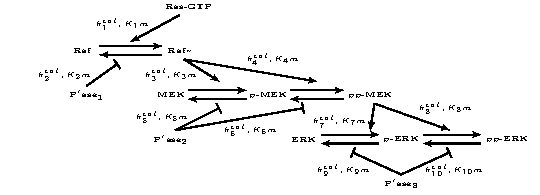
\includegraphics[clip=true, width=0.5\textwidth]{Figure_3.pdf}
    }

    \subfigure[] {
        \label{fig:example_reis_interdisciplinary:B}
        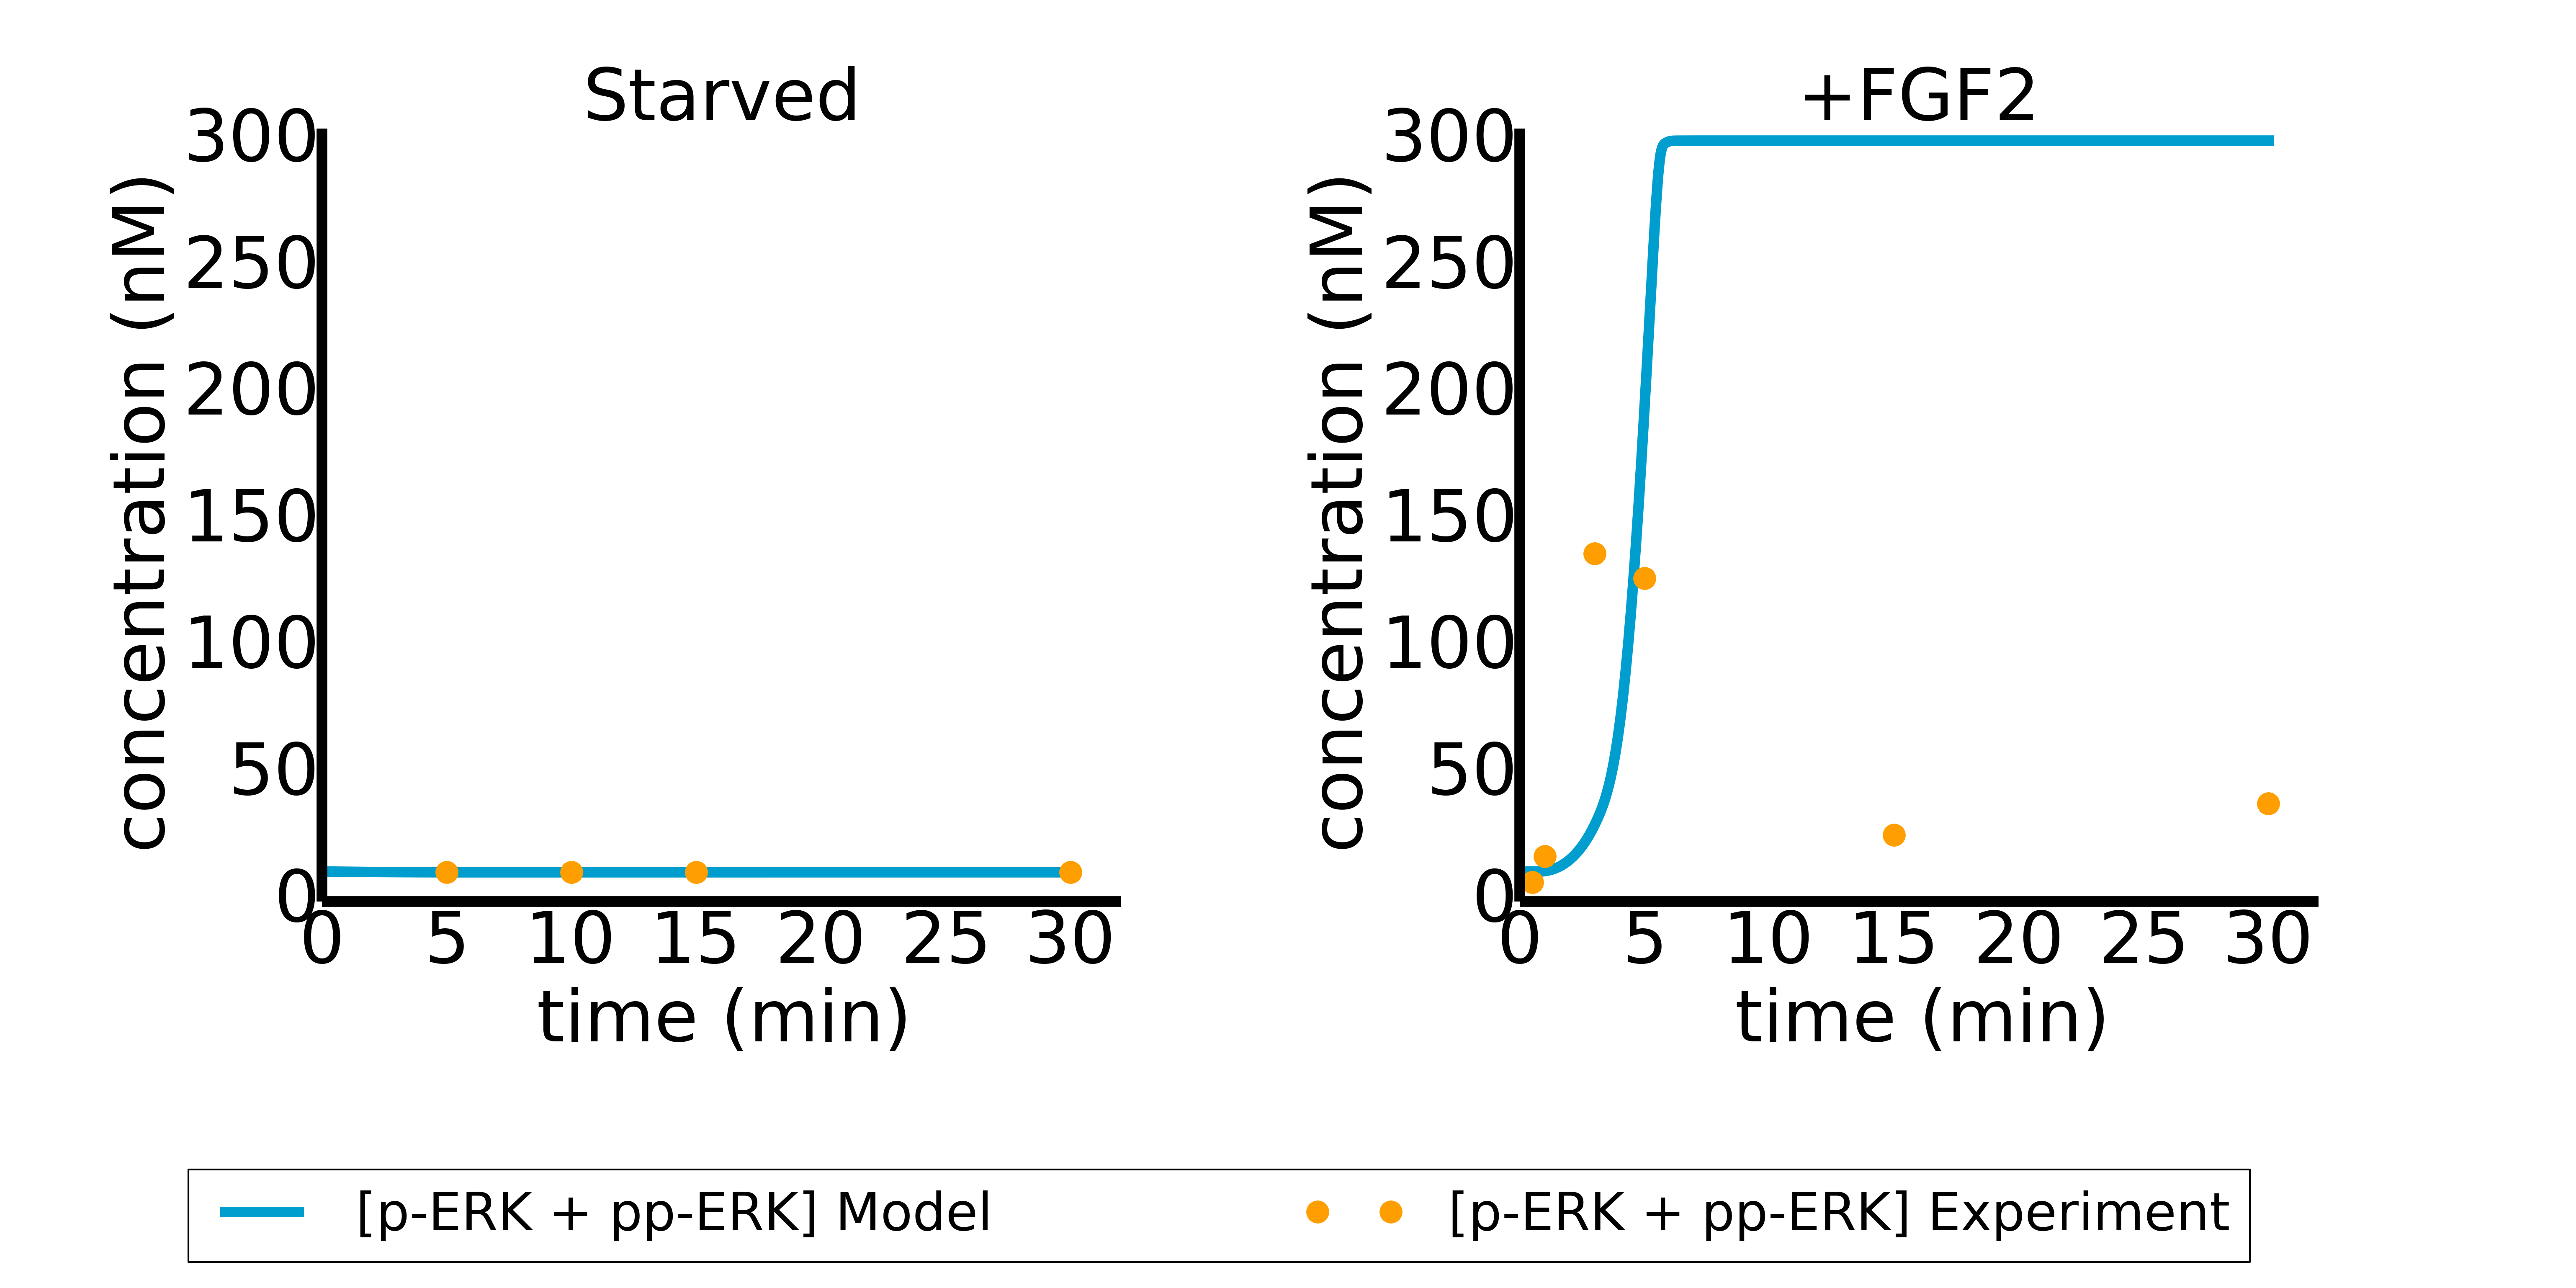
\includegraphics[clip=true, width=0.5\textwidth]{Figure_5.png}
    }
    \subfigure[] {
        \label{fig:example_reis_interdisciplinary:C}
        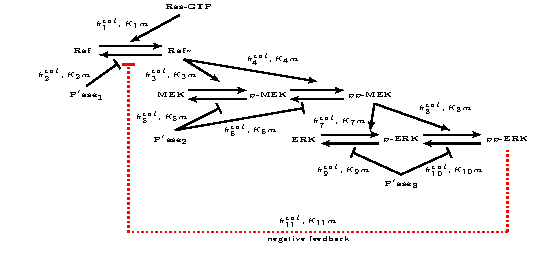
\includegraphics[clip=true, width=0.5\textwidth]{Figure_6.pdf}
    }
    \subfigure[] {
        \label{fig:example_reis_interdisciplinary:D}
        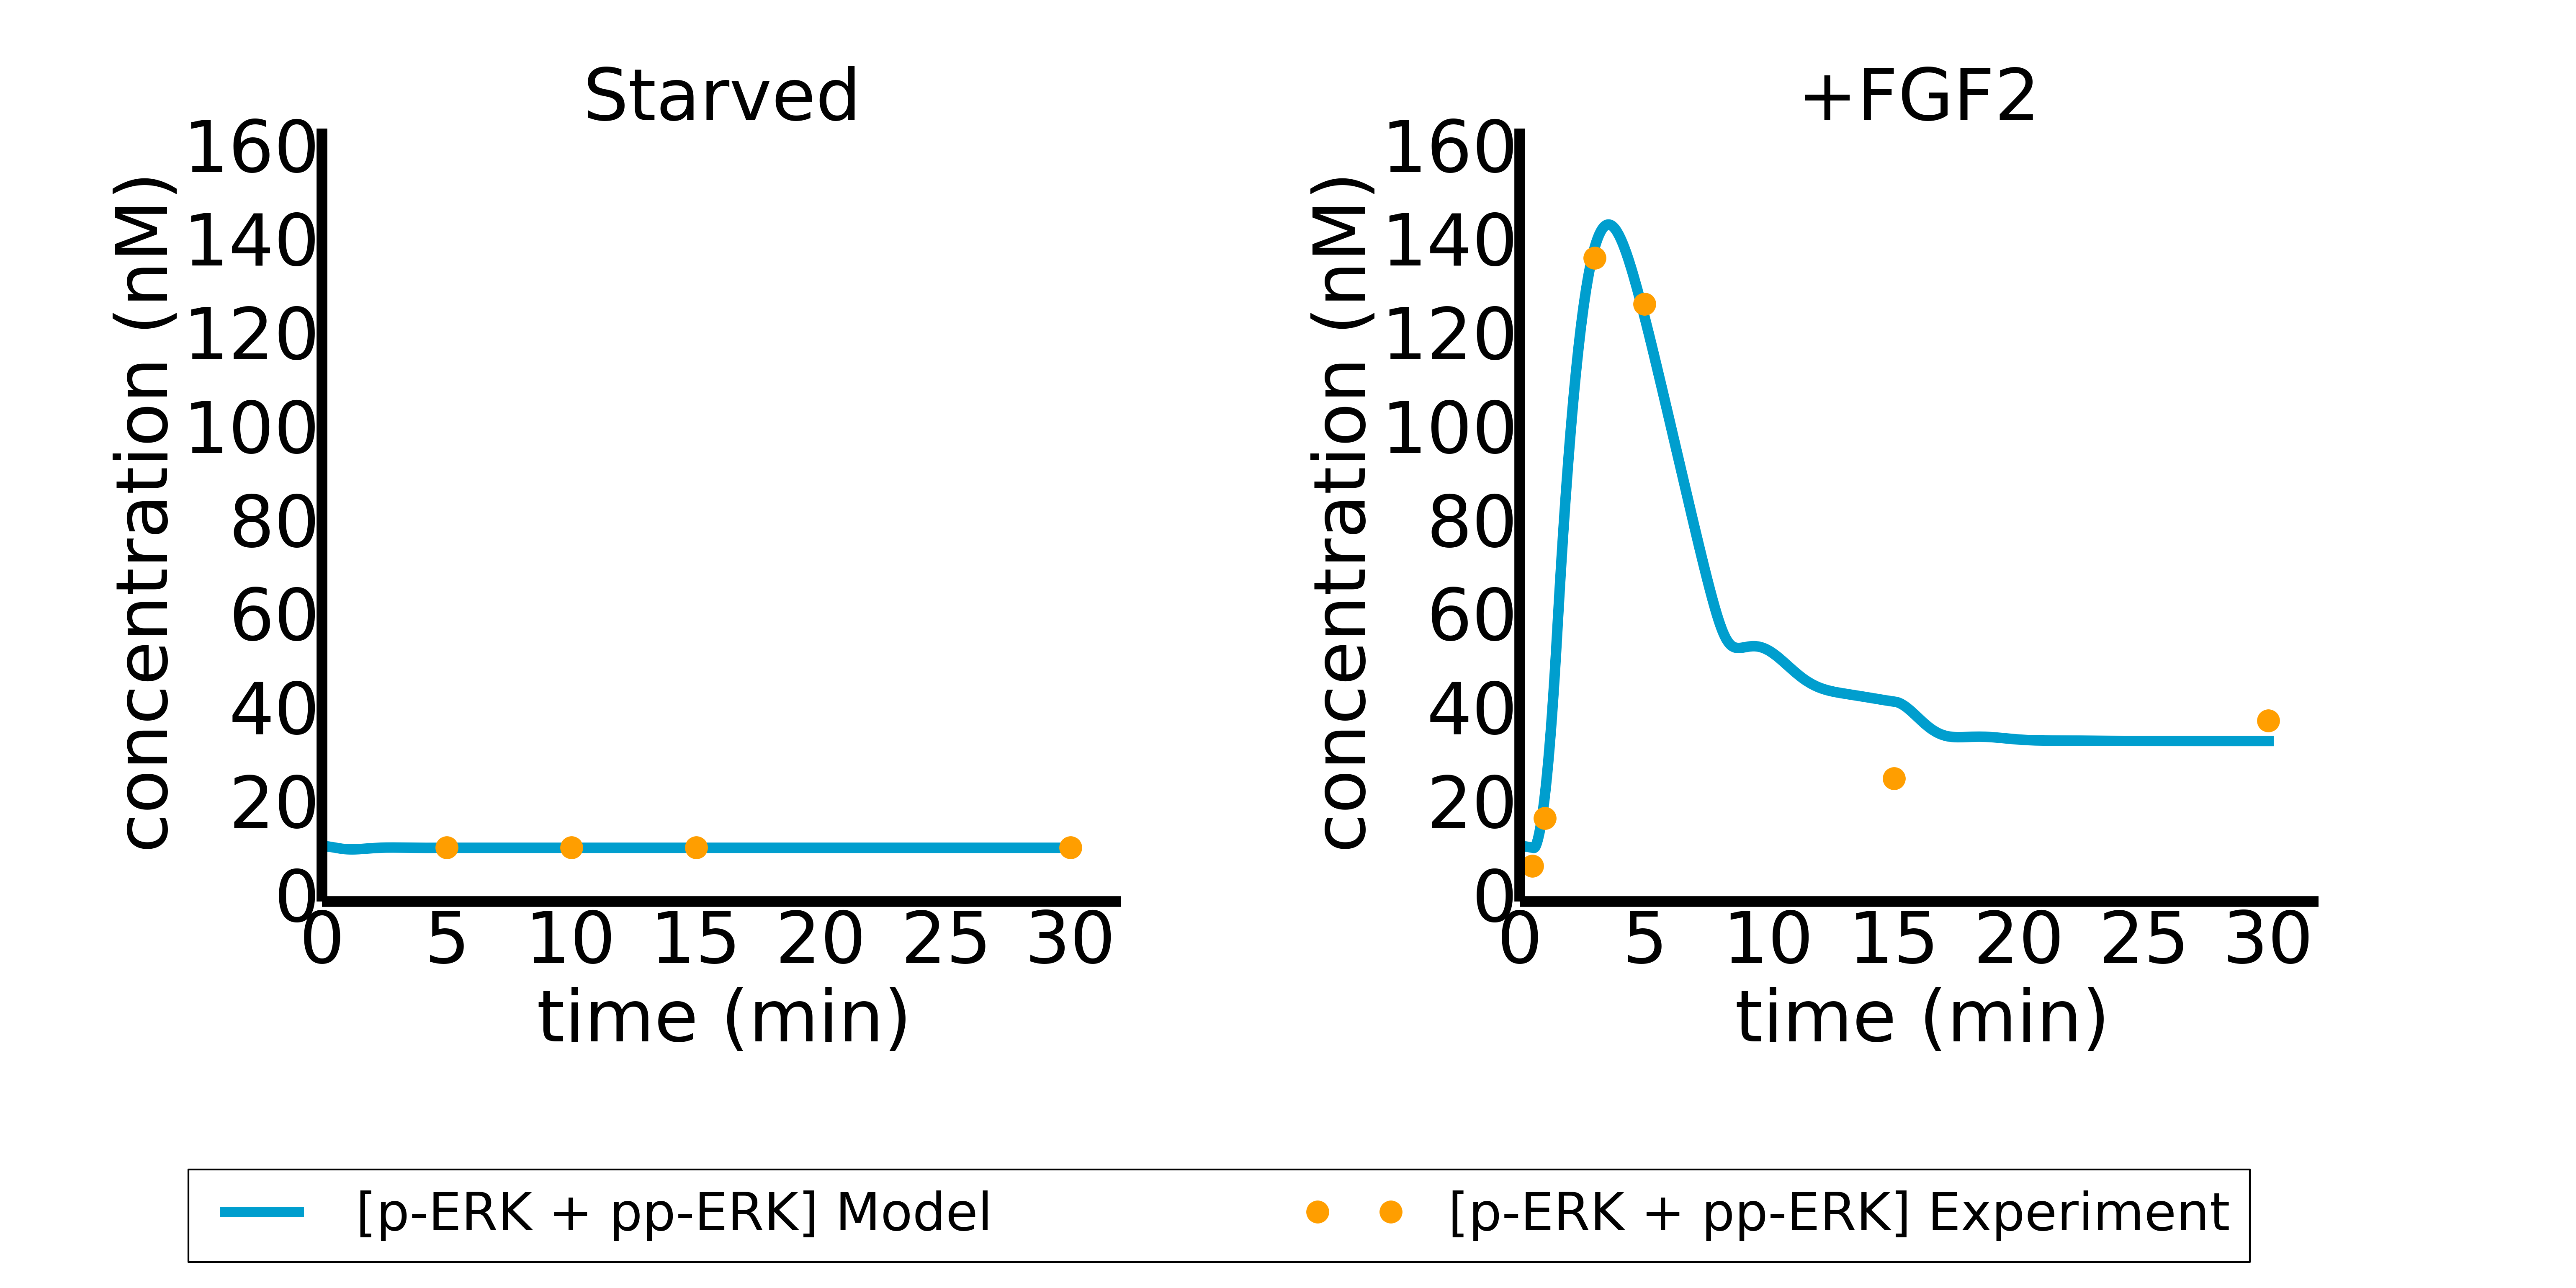
\includegraphics[clip=true, width=0.5\textwidth]{Figure_7.png}
    }
        
    \caption{Exemplo de identificação da via de sinalização Ras/ERK em
    células carcinoma adrenocorticais Y1 de rato 
    ~\cite{Reis2017interdisciplinary}. As figuras 
    \ref{fig:example_reis_interdisciplinary:A} e 
    \ref{fig:example_reis_interdisciplinary:C} representam 
    respectivamente o modelo funcional e um gráfico comparando dados da
    simulação e do experimento biológico. O gráfico mostra que a 
    simulação não se aproxima bem da realidade, o que é contornado por
    Reis et al. adicionando uma nova interação no modelo funcional 
    (em vermelho na figura \ref{fig:example_reis_interdisciplinary:B})
    . O modelo atualizado e os resultados da simulação são apresentados
    respectivamente nas figuras 
    \ref{fig:example_reis_interdisciplinary:B} e
    \ref{fig:example_reis_interdisciplinary:D}} 
    \label{fig:example_reis_interdisciplinary} 
\end{figure}
\FloatBarrier

% 3 limitações
% penalização
% completude
% apenas incremental

\subsection{Modificação de modelos funcionais a partir de bancos de 
dados de interatomas}
Com intuito de sistematizar a modificação de um modelo funcional, foi
desenvolvido em uma tese de mestrado uma abordagem de identificação de
vias de sinalização celular que aumenta recortes de mapas de interatomas
com o objetivo de que o modelo represente corretamente os dados biológicos 
~\cite{Wu2015metodo}. Esta abordagem modifica os modelos funcionais de 
forma incremental, adicionando interações de um banco de dados, que foi 
construído com a união de várias interações de diferentes mapas de 
interatomas do KEGG.

Mais formalmente, esta abordagem trata o problema de identificação de 
vias de sinalização como um problema de otimização, em que o espaço de
busca é constituído por todos os modelos que podem ser construídos a 
partir do modelo original (incluindo ele mesmo), aumentado com
interações do banco de dados usado. A função de custo é dada pelo erro
do modelo no ajuste de curva dos dados biológicos, calculado pelo 
software SigNetSim; a busca pelo melhor elemento do espaço de busca é 
feita usando o algoritmo de busca {\it Sequential Forward Selection} 
(SFS).

% TODO: descobrir outros bancos de mapas interatomas 

Esta abordagem, entretanto, apresentou algumas limitações. A primeira é 
a incompletude do banco de interações criado, que usava apenas mapas de 
interatomas disponíveis no KEGG e, além disso, não considera constantes 
de velocidade disponíveis em outros bancos de dados, como o 
Sabio-RK~\cite{doi:10.1093/nar/gkr1046}, 
o que aumenta desnecessariamente a complexidade do modelo 
funcional. A segunda limitação está no algoritmo de busca, que por ser
incremental pode ``caminhar'' o modelo até um mínimo local, perdendo a 
melhor solução. A terceira e última está na penalização de modelos mais 
complexos, que era feita implicitamente ao impor um tempo de limite 
no ajuste de curva do modelo, ignorando a velocidade de convergência do
algoritmo para o modelo em questão, resultando em uma penalização 
aleatória.

%\begin{itemize}

%\item Enunciar o problema de identificação de vias de sinalização celular. Ilustrá-lo utilizando o exemplo do paper da Methods in Molecular Biology~\cite{Reis2017interdisciplinary}. Para isto monte uma figura com 4 subfiguras, mostrando a simulação do modelo inicial, e depois com o acréscimo de uma reação (os arquivos das subfiguras estão na pasta ``figures").

%\item Explicar, de forma concisa, a abordagem da Lulu para tentar resolver o problema~\cite{Wu2015metodo}, que envolve o uso do repositório de interatomas KEGG~\cite{Kanehisa2000kegg}. Citar limitações dessa abordagem, como por exemplo o uso do SFS como função custo para fazer a seleção de modelos~\cite{Whitney:1971}.

%\end{itemize}

%------------------------------------------------------------------------------%

\section{Objetivos}

\begin{itemize}

\item \underline{Geral:} desenvolver uma abordagem mais efetiva para auxiliar na identificação de vias de sinalização celular. Esta abordagem teria como ponto de partida o trabalho da Lulu e incluiria soluções para as limitações do mesmo, que foram discutidas na seção anterior.

\item \underline{Específico:} aplicar a metodologia na identificação de vias de sinalização celular relevantes em nosso estudo de caso, a linhagem tumoral murina Y1.

\end{itemize}

%------------------------------------------------------------------------------%

\section{Metodologia}



\subsection{Desafios científicos}

\begin{enumerate}

\item Realizar a seleção de modelos utilizando uma estratégia global ao invés de incremental. Para este fim, faremos a redução do problema da seleção de modelos para um problema de seleção de características, o que exigirá:
\begin{itemize}
  \item Definir uma função custo apropriada, que leve em consideração a penalização por {\em overfitting} decorrente do acréscimo de novas espécies químicas e/ou reações sem a inclusão de novas medidas experimentais para ajustar o modelo aumentado. Uma possibilidade seria o uso do critério de informação de Akaike ({\em Akaike's Information Criterion} -- AIC)~\cite{bozdogan1987model}, cujo princípio foi aplicado com sucesso em seleção de modelos no contexto de discriminação de classes de redes biológicas~\cite{takahashi2012discriminating}. Também investigaremos para este fim o uso de abordagens Bayesianas~\cite{kirk2013model}, como por exemplo a técnica conhecida como {\em Bayesian inference-based modeling} (BIBm)~\cite{Xu2010}.

  \item Escolher um algoritmo de seleção de características. Critérios que penalizam {\em overfitting} provavelmente induzirão curvas em U nas cadeias do reticulado Booleano induzido pelo espaço de busca, o que nos permitirá aproximar o problema de seleção de características através do problema de otimização U-curve. Como o cálculo da função custo provavelmente será computacionalmente muito intensivo, o melhor algoritmo para esse fim tende a ser o U-Curve-Search (UCS)~\cite{reis2012minimizaccao,reis2017ucsr}.
\end{itemize}

\item Contornar o problema da incompletude dos bancos de dados de interatomas (e.g., KEGG), que se dá no nível de estrutura da via de sinalização e também na ausência de constantes de velocidade.
  \begin{itemize}
     \item{\bf Estrutura da via de sinalização.} \href{http://www.genome.jp/kegg-bin/show\_pathway?mmu04014}{no mapa da via de sinalização de Ras em camundongo}, existe uma aresta dizendo que Raf1 ativa MEK, mas não como se dá tal ativação. Por exemplo, no modelo apresentado na introdução, MEK é ativado após ser fosforilado duas vezes pela forma ativa de Raf1, dinâmica que exige duas equações para ser descrita em termos de cinética química. Para lidar com este problema, precisaremos estabelecer a lei cinética (tipo de reação) a ser utilizada de acordo com a natureza das espécies químicas envolvidas em uma dada interação. No exemplo dado, sabe-se que a ativação de MEK por Raf é ultrassensível, e que portanto pode ser modelada utilizando a equação de Hill~\cite{huang1996ultrasensitivity}.
     \item{\bf Ausência de constantes de velocidade.} Dificulta tanto a estimação quanto o problema de otimização. Vamos contornar isso coletando e organizando informações extraídas de repositórios tais como o Sabio-RK~\cite{doi:10.1093/nar/gkr1046}, Brenda~\cite{doi:10.1093/nar/gkh081}, BioNumbers~\cite{milo2009bionumbers}, e possivelmente também  BioModels~\cite{le2006biomodels}. 
  \end{itemize}
\end{enumerate}


\subsection{Desafios tecnológicos}

\begin{enumerate}

% Obs: o primeiro item já estamos adiantando com os trabalhos para o X-Meeting 2017.
%
\item Integração apropriada do featsel~\cite{Reis2017featsel} com o SigNetSim~\cite{Noel2017SigNetSim} para seleção de modelos.

\item Organização das informações coletadas em um banco de dados relacional, que será integrado ao \href{http://cetics.butantan.gov.br/ceticsdb/accounts/login/?next=/ceticsdb/}{CeTICSdb}, repositório de ômicas desenvolvido e mantido pelo grupo de Biologia Computacional do CeTICS.

\end{enumerate}

%------------------------------------------------------------------------------%

\section{Plano de trabalho e cronograma de execução}

{\color{blue}[Tente detalhar os trabalhos que serão necessários, dados os objetivos e desafios metodológicos.]}

\subsection{Cronograma proposto}

{\color{blue}[Tabela análoga ao dos projetos anteriores.]}

%------------------------------------------------------------------------------%

\section{Forma de análise e disseminação de resultados}

{\color{blue}[Análogo ao nosso último projeto.]}

%------------------------------------------------------------------------------%

\addcontentsline{toc}{section}{Referências}
\bibliographystyle{unsrt} 
\bibliography{bib-proposta-MSc-gestrela}

\end{document}

